\documentclass[french]{article}
    \usepackage[T1]{fontenc}
    \usepackage[utf8]{inputenc}
    \usepackage{lmodern}
    \usepackage[a4paper]{geometry}
    \usepackage{babel}
    \usepackage{bm}
    \usepackage{enumitem}
    \usepackage{xcolor}
    \usepackage{amsmath} 
    \usepackage{amssymb}  
    \usepackage{gensymb}
    \usepackage{graphicx}
    \newcommand*{\norme}[1]{\left\lVert{#1}\right\rVert}
	
	\title{Note de machine learning}
	\author{DJEBALI Wissam}
    
    \begin{document}	
    \maketitle
%%%%%%%%%%%%%%%%%%%%%%%%%%%%%%%%%%%%%%%%%%%%%%%%%%%%%%%%%%%%%%%%%%%%%%%%%%%%%%%%%%%%%%%
%%%%%%%%%%%%%%%%%%%%%%%%%%%%%%%%%%%%%%%%%%%%%%%%%%%%%%%%%%%%%%%%%%%%%%%%%%%%%%%%%%%%%%%    
	\section{Traiter les valeurs manquantes(à compléter)}
	\subsection{Variables quantitatives}
Deux solutions existent pour traiter les valeurs manquantes : 
	\begin{itemize}[label=\textbullet, font=\LARGE \color{orange}]
		\item Supprimer les individus avec des valeurs manquantes
		\item Remplacer les valeurs manquantes par d'autres valeurs. Il faut alors veiller à ne pas modifier la distribution de la variable en question, conserver le plus de propriétés de celle-ci.
		\begin{itemize}[label=*]
			\item On peut remplacer les valeurs manquantes par la médiane, la moyenne(déconseillée) ou d'autre valeurs
			\item On peut aussi utiliser des algorithmes afin de remplacer ses valeurs manquantes de façon plus judicieuses, ces algorithmes sont appelés \textbf{Algorithm for Impute Values}
		\end{itemize}
	\end{itemize}
	
%%%%%%%%%%%%%%%%%%%%%%%%%%%%%%%%%%%%%%%%%%%%%%%%%%%%%%%%%%%%%%%%%%%%%%%%%%%%%%%%%%%%%%%
%%%%%%%%%%%%%%%%%%%%%%%%%%%%%%%%%%%%%%%%%%%%%%%%%%%%%%%%%%%%%%%%%%%%%%%%%%%%%%%%%%%%%%%
	
	\section{Cross Validation}
	(à compléter)
%%%%%%%%%%%%%%%%%%%%%%%%%%%%%%%%%%%%%%%%%%%%%%%%%%%%%%%%%%%%%%%%%%%%%%%%%%%%%%%%%%%%%%%
%%%%%%%%%%%%%%%%%%%%%%%%%%%%%%%%%%%%%%%%%%%%%%%%%%%%%%%%%%%%%%%%%%%%%%%%%%%%%%%%%%%%%%%
	
    \section{Loss Functions}
    \subsection{Loss Functions}
    $\bm{y}$ est la vraie valeur et $\bm{y'}$ est la valeur prédite.\\
    \begin{itemize}[label=\textbullet, font=\LARGE \color{red}]
        \item $\bm{L_{\textbf{0-1}}(y,y')=\mathbb{I}_{yy'\leq 0}}$
        \item $\bm{L_{\textbf{hinge}}(y,y')=(1-yy')_{+}}$
        \item $\bm{L_{\textbf{logistic}}(y,h(x))=Log_{\textbf{loss}}(y,h(x))=log(1+e^{-y\times h(x)})=\sum_{(x,y)\in D}-y\log(h(x))-(1-y)\log(1-h(x))}$
        \item $\bm{L_{\textbf{Quadratic Hingle Loss}}(y,y')=\frac{1}{2}(1-yy')^{2}_{+}}$
        \item $\bm{L_{\textbf{Huber loss}}(y,y') = -4yy'\mathbb{I}_{yy'\le -1} + (1-yy')^{2}_{+}\mathbb{I}_{yy'\geq-1}}$
        \item $\bm{L_{\textbf{least-squares}}(y,y')=\frac{1}{2}(y-y')^{2}}$ (régression linéaire)
    \end{itemize}
    
    \subsection{Loss Functions with Regularization}

	Au lieu de seulement chercher à minimiser la perte (minimisation du risque empirique), comme suit : 
$$\bm{minimiser(Perte(Données|Modèle))}$$
Pour éviter le \textbf{surapprentissage(overfitting)}, nous allons minimiser à la fois la perte et la complexité, ce qui s'appelle la \textbf{minimisation du risque structurel} : 
$$\bm{minimiser(Perte(Données|Modèle))+complexité(Modèle)}$$
Notre algorithme d'optimisation de l'apprentissage est désormais une fonction à deux facteurs : le \textbf{facteur de perte}, qui mesure l'efficacité d'apprentissage du modèle, et le \textbf{facteur de régularisation}, qui mesure la complexité du modèle.\\\\
Il y a deux façon courantes(et apparentées) d'aborder la complexité d'un modèle : 
\begin{itemize}[label=\textbullet]
\item La complexité du modèle en tant que fonction des pondérations de toutes les caractéristiques du modèle.
\item a complexité du modèle en tant que fonction du nombre total de caractéristiques dont les pondérations sont différentes de zéro
\end{itemize}

Si la complexité du modèle est fonction des pondérations, la pondération d'une caractéristique est plus ou moins complexe selon que sa valeur absolue est plus ou moins élevée.\\\\
\begin{itemize}[label=\textbullet, font=\LARGE \color{red}]

\item \textbf{Régression Ridge(Régression avec pénalisation(régularisation) norme $L_{2}$}

Nous pouvons quantifier la complexité à l'aide de la formule de 
$\bm{L_2}$, qui définit le facteur de régularisation comme étant la somme des carrés de toutes les pondérations des caractéristiques :	
$$L_{2}\text{\textbf{ facteur de régularisation}}=||w||^{2}_{2} = w^{2}_{1}+w^{2}_{2}+w^{2}_{3}+...+w^{2}_{n}$$
Dans cette formule, les pondérations proches de zéro ont peu d'effet sur la complexité du modèle, tandis que celles qui correspondent à des anomalies peuvent avoir un effet considérable.\\\\
Les développeurs de modèles ajustent l'effet global du facteur de régularisation en multipliant sa valeur par une grandeur scalaire appelé \textbf{lambda}(ou \textbf{taux de régularisation}). Ils cherchent à obtenir le résultat suivant: 
	$$\bm{minimiser(Perte(Données|Modèle)+\lambda complexité(Modèle))}$$
Avec la régularisation $L_{2}$ on veut  : $$\bm{min(func_{Loss}+\lambda ||w||^{2}_{2})}$$
La régularisation $L_{2}$ a les effets suivants sur un modèle : 
\begin{itemize}[label=\textbullet]
\item Les valeurs des pondérations se rapprochent de (mais ne sont pas exactement égales à) zéro.
\item a moyenne des pondérations tend vers zéro, avec une distribution normale (en cloche ou gaussienne).
\end{itemize}
L'augmentation du lambda renforce les effets de la régularisation.\\\\
Le lambda choisi doit permettre d'obtenir un juste équilibre entre simplicité et efficacité d'apprentissage :
\begin{itemize}[label=\textbullet]
\item Si le lambda est trop élevé, le modèle sera simple, mais il présentera un risque de sous-apprentissage des données. Le modèle n'en apprendra pas suffisamment sur les données d'apprentissage pour réaliser des prédictions utiles.
\item Si le lambda est trop faible, le modèle sera plus complexe, et il présentera un risque de surapprentissage des données. Le modèle apprendra trop sur les spécificités des données d'apprentissage, et il ne pourra pas généraliser celles-ci à de nouvelles données.
\end{itemize}


\paragraph{Remarque : } 
La définition du lambda sur zéro supprime complètement la régularisation. Dans ce cas, l'apprentissage vise exclusivement à minimiser la perte, et le risque de surapprentissage est maximal.\\\\

Le lambda idéal produit un modèle qui effectue une généralisation efficace en cas de nouvelles données qui n'étaient pas visibles précédemment. Le lambda idéal dépend des données, on doit donc malheureusement procéder à des réglages.


\item \textbf{Régression LASSO(Régression avec pénalisation(régularisation) norme $L_{1}$}

Même principe que la \textbf{Régression Ridge} mais en utilisant la \textbf{norme} $\bm{L_{1}}$. C'est une pénalisation plus sévère que \textbf{Ridge}\\.

Avec la régularisation $L_{1}$ on veut  : $$\bm{min(func_{Loss}+\lambda ||w||_{1})}$$
La régularisation $L_{1}$ a les effets suivants sur un modèle : 
\begin{itemize}[label=\textbullet]
\item Fixe les valeurs de certaines pondérations à zéro.
\item Supprime le poids de certaines variables dans le modèle.
\end{itemize}

Pour le reste on retrouve les mêmes interprétations.\\

\textbf{A noter que les normes $L_{1}$ et $L_{2}$ permettent de garder un problème convexe et donc résolvable.}\\

\subsubsection{Remarque : \\}

\begin{itemize}
	
	\item[$\star$] La dérivée de $\bm{L_{2}}$ est comparable à une force qui retire x \% de la pondération à chaque fois. Comme le savait Zénon, même si vous retirez x \% d'un nombre plusieurs milliards de fois, le nombre ainsi réduit ne sera jamais égal à 0. (Zénon n'était pas conscient de la précision limitée des calculs en virgule flottante, qui peuvent produire un résultat exactement égal à 0). Quoi qu'il en soit, la régularisation $\bm{L_{2}}$ ne ramène généralement pas les pondérations à 0.\\
	
	\item[$\star$] La dérivée de $\bm{L_{1}}$ est comparable à une force qui soustrait une constante de la pondération à chaque fois. Toutefois, grâce aux valeurs absolues, $\bm{L_{1}}$ présente une discontinuité à 0, si bien que les résultats de la soustraction qui sont inférieurs à 0 sont mis à 0. Par exemple, si la soustraction fait passer une pondération de +0,1 à -0,2, $\bm{L_{1}}$ définit cette pondération sur exactement 0. $\bm{L_{1}}$ met donc la pondération à 0, ce qui correspond exactement au but recherché.\\\\En pénalisant la valeur absolue de toutes les pondérations, la régularisation $\bm{L_{1}}$ s'avère particulièrement efficace pour les modèles larges.\\
\end{itemize}
 


\item \textbf{ElasticNet}\\
Combinaison des fonction de \textbf{la Régression Ridge} et de la \textbf{Régression LASSO}.

\end{itemize}

%%%%%%%%%%%%%%%%%%%%%%%%%%%%%%%%%%%%%%%%%%%%%%%%%%%%%%%%%%%%%%%%%%%%%%%%%%%%%%%%%%%%%%%
%%%%%%%%%%%%%%%%%%%%%%%%%%%%%%%%%%%%%%%%%%%%%%%%%%%%%%%%%%%%%%%%%%%%%%%%%%%%%%%%%%%%%%%
	
    \section{Kernel(Utilisés dans SVM)}
    \begin{itemize}[label=\textbullet, font=\LARGE \color{red}]
        \item \textbf{The RBF Kernel}(Radial Basis Function)\\
        Pour $\gamma>0$ $$\bm{K(x,x') = \exp(-\gamma\norme{x-x}^{2}_{2})}$$ 
        \item \textbf{The Tanh Kernel} aussi appelé \textbf{The Sigmoid Kernel}\\
        $$\bm{K'(x,x')=tanh(a\langle x,x'\rangle + c) = \frac{e^{a\langle x,x'\rangle + c}-e^{a\langle x,x'\rangle - c}}{e^{a\langle x,x'\rangle + c}+e^{a\langle x,x'\rangle - c}} \text{ pour } a>0,c>0}$$
    \end{itemize}

%%%%%%%%%%%%%%%%%%%%%%%%%%%%%%%%%%%%%%%%%%%%%%%%%%%%%%%%%%%%%%%%%%%%%%%%%%%%%%%%%%%%%%%
%%%%%%%%%%%%%%%%%%%%%%%%%%%%%%%%%%%%%%%%%%%%%%%%%%%%%%%%%%%%%%%%%%%%%%%%%%%%%%%%%%%%%%%
	
	\section{Fonctions Distances: }
	\begin{itemize}[label=\textbullet, font=\LARGE \color{red}]
		\item \textbf{Distance Euclidienne}
		$$\bm{d(x_{1},x_{2})=\sqrt{\sum_{j=1}^{n}(x_{1j}-x_{2j})^{2}}}$$
		
		\item \textbf{Distance chi-deux}
		$$\bm{d(x_{1},x_{2})=\sqrt{\sum_{j=1}^{n}\frac{1}{f_{n}}(f_{1j}-f_{2j})^{2}}}$$
		avec $f_{ij}$ proportion par individu et $f_{j}$ proportion moyenne pour la variable j.\\
		
		\item \textbf{Distance de Manhattan(ou distance City-Block ou Taxi-Distance)}
		$$\bm{d(x_{1},x_{2})=\sum_{j=1}^{n}|x_{1j}-x_{2j}|}$$
		Par rapport à la distance euclidienne usuelle, qui utilise le carré des écarts, on utilisera notamment cette mesure pour minimiser l’influence des grands écarts.\\
		
		\item \textbf{Distance de Gower} = métrique utilisée dans le Clustering pour des
jeux de données mixtes (contenant des variables quantitatives et qualitatives). Permet de faire d'utiliser des Clustering prenant à la fois en compte les données quantitatives et qualitatives(\textit{cf Kmodes})
	\end{itemize}
%%%%%%%%%%%%%%%%%%%%%%%%%%%%%%%%%%%%%%%%%%%%%%%%%%%%%%%%%%%%%%%%%%%%%%%%%%%%%%%%%%%%%%%
%%%%%%%%%%%%%%%%%%%%%%%%%%%%%%%%%%%%%%%%%%%%%%%%%%%%%%%%%%%%%%%%%%%%%%%%%%%%%%%%%%%%%%%
	
	\section{Fonctions Sigmoïde(utilisées dans Régression Logistique,...)}
	\begin{itemize}[label=\textbullet, font=\LARGE \color{red}]
		\item \textbf{Courbe de Gompertz : }
			$$\bm{y(t)=a\exp(-be^{-ct})}$$
			La courbe de Gompertz est utilisée pour modéliser certaines séries temporelles, dont la
			croissance est lente au départ et s’arrête à un moment. Cette fonction est employée pour
			décrire une population dans un espace confiné, dont la reproduction augmente au début
			puis ralenti une fois que les ressources à disposition deviennent rares 1.
			
		\item \textbf{tangente hyperbolique :}
		$$\bm{tanh(t)=\frac{e^{t}-e^{-t}}{e^{t}+e^{-t}}}$$
		Bien que la tangente hyperbolique soit à la base une fonction complexe, on s’intéresse ici
		à sa restriction à , qui est une bijection strictement croissante de dans [-1,1].
		
		\item \textbf{Fonction de répartition de la loi normale centrée réduite :}
		$$\bm{\phi(t)=\frac{1}{\sqrt{2\pi}}\int^{t}_{-\infty}e^{-\frac{1}{2}x^{2}}dx}$$
		
	Les fonctions de répartition de la loi de normale centrée réduite sont de magnifiques
	candidates pour la fonction hypothèse que l’on recherche. Dans les faits, on préférera la
	fonction de répartition de la loi logistique.
	
	\item \textbf{Fonction de répartition de la loi logistique :}
	$$\bm{g(t,\mu,s)=\frac{1}{1+e^{-\frac{t-\mu}{s}}}}$$
	La loi logistique ressemble beaucoup à une loi normale, mais elle présente un plus grand
	kurtosis (indicateur qui mesure le coefficient d’applatisssement d’une distribution).\\
	
	\textbf{Cas particulier : Fonction logistique}\\
	Un cas particulier de la fonction de répartition de la loi logistique est celle de paramètre
	(0,1). On l’appelle fonction logistique et elle se définit comme suit : $$\bm{g(t)=\frac{1}{1+e^{-t}}}$$
	On nommera fonction sigmoïde cette fonction logistique. Elle est effectivement, dans la littérature et la pratique, la fonction sigmoïde la plus utilisée.
	\end{itemize}
	
%%%%%%%%%%%%%%%%%%%%%%%%%%%%%%%%%%%%%%%%%%%%%%%%%%%%%%%%%%%%%%%%%%%%%%%%%%%%%%%%%%%%%%%
%%%%%%%%%%%%%%%%%%%%%%%%%%%%%%%%%%%%%%%%%%%%%%%%%%%%%%%%%%%%%%%%%%%%%%%%%%%%%%%%%%%%%%%
	
	\section{Régression}
Soient un ensemble de $\bm{m}$ variables $\bm{X_{1},X_{2},...,X_{m}}$ pour lesquelles on possède $\bm{n}$ observations, le tout représenté dans la matrice $\bm{X}$. On souhaite à partir des variables $\bm{X_{1},X_{2},...,X_{m}}$ et leurs observations prédire la variable $\bm{Y}$. On cherche donc une fonction de la forme : 
$$
\bm{\hat{Y}=f(X)=wX+b=w_{1}X_{1}+w_{2}X_{2}+...+w_{m}X_{m}+b}
$$
tel que $\bm{\hat{Y}}$ qui est le vecteur des valeurs prédites se rapproche le plus possible du vecteur des valeurs cibles $\bm{Y}$
\begin{itemize}[label = \textbullet]
	\item $\bm{w}$ représente le vecteur des poids
	\item \textbf{le biais} est défini par $\bm{Y-wX-b}$.
	\item $\bm{b}$ est l'ordonnée à l'origine appelé aussi \textbf{intercept}.
	\item l'erreur est donnée par : $\bm{Y-\hat{Y}=Y-f(X)=Y-wX-b}$.\\
	On utilise jamais l'erreur tel quelle, on préfère considérait la somme du carrés erreurs : 
	$$\sum_{i=1}^{n}(f(X^{i})-Y^{i})^{2}$$  
\end{itemize}
%%%%%%%%%%%%%%%%%%%%%%%%%%%%%%%%%%%%%%%%%%%%%%%%%%%%%%%%%%%%%%%%%%%%%%%%%%%%%%%%%%%%%%%
%%%%%%%%%%%%%%%%%%%%%%%%%%%%%%%%%%%%%%%%%%%%%%%%%%%%%%%%%%%%%%%%%%%%%%%%%%%%%%%%%%%%%%%	
	
	\section{Classification}
	\subsubsection{Justesse}
	$$\bm{Justesse=\frac{\text{Nombre de prédictions correctes}}{\text{Nombre total de prédictions}}}$$
	\subsubsection{Précision, Rappel}
	$$\bm{Precision = Precision =\frac{VP}{VP+FP}}$$
	où \textbf{VP = Vrais Positifs} et \textbf{FP = Faux Positifs}
	$$\bm{Rappel = Recall = \frac{VP}{VP+FN}}$$
	où \textbf{FN = Faux Négatifs}
	\subsubsection{Courbe ROC(Receiver Operating Characteristic)}
	$$\bm{\text{\textbf{Taux de vrais positifs}}=\frac{VP}{VP+FN}=Recall}$$
	$$\bm{\text{\textbf{Taux de faux positifs}}=\frac{FP}{FP+VN}}$$
	$$\bm{\text{\textbf{Courbe ROC}}:\{\text{\textbf{Taux de VP=Recall}}=func(\text{\textbf{Taux de FP}})}\}$$
	
	\subsubsection{Biais de Prédiction}
	\begin{center}
		\textbf{biais de prédiction = valeur moyenne des prédictions - valeur moyenne des étiquettes dans l'ensemble des données}
	\end{center}
Un biais de prédiction très différent de zéro vous informe que votre modèle ne fonctionne pas correctement, puisqu'il n'identifie pas la fréquence réelle des étiquettes positives.\\

Admettons, par exemple, que nous savons que 1 \% de tous les e-mails sont du spam. Si nous ignorons tout d'un e-mail donné, nous devrions prédire que la probabilité pour qu'il s'agisse de spam est de 1 \%. Selon cette logique, un bon modèle de détection de spam doit prédire en moyenne que les e-mails ont 1 \% de chances d'être du spam. En d'autres termes, si nous calculons la moyenne des prédictions de probabilité pour que chaque e-mail soit du spam, le résultat devrait être 1 \%. Mais si la prédiction moyenne du modèle évalue la probabilité du spam à 20 \%, nous pouvons en conclure que le modèle est affecté d'un biais de prédiction.\\\\
Plusieurs causes peuvent être à l'origine d'un biais de prédiction :
\begin{itemize}[label=\textbullet]
	\item Un ensemble de caractéristiques incomplet
	\item La présence de bruit dans l'ensemble de données
	\item Un pipeline ne fonctionnant pas correctement
	\item Un échantillon d'apprentissage non représentatif
	\item Une régularisation excessive\\
\end{itemize}
Vous pourriez être tenté de corriger un \textbf{biais de prédiction} en ajustant le modèle après apprentissage, c'est-à-dire en ajoutant un niveau de calibration afin d'adapter les résultats de votre modèle et de diminuer le biais de prédiction.\\ 
Par exemple, si votre modèle a un biais de prédiction de +3 \%, vous pouvez ajouter un nouveau de calibration réduisant la prédiction moyenne de 3 \%.\\
Toutefois, l'ajout d'un niveau de calibration est déconseillé pour les raisons suivantes :
\begin{itemize}[label=\textbullet]
	\item Vous intervenez sur le symptôme et non sur la cause du biais.
	\item Votre système devient moins flexible et requiert désormais d'être tenu à jour.\\
\end{itemize}
Dans la mesure du possible, évitez les niveaux de calibration. Les projets qui ont recours aux niveaux de calibration ont tendance à en devenir dépendants, car ils les utilisent pour résoudre tous les défauts de leur modèle. La gestion de tous ces niveaux de calibration peut finir par tourner au cauchemar.

\paragraph{Remarque:}
Un bon modèle aura généralement un \textbf{biais de prédiction} voisin de zéro. Cela étant, un \textbf{biais de prédiction} très bas ne suffit pas à garantir la qualité de votre modèle. Un très mauvais modèle peut avoir un \textbf{biais de prédiction} négligeable. Par exemple, un modèle prédisant simplement la valeur moyenne pour tous les exemples serait un mauvais modèle, malgré un \textbf{biais de prédiction} égal à zéro.

	\subsubsection{Régression logistique}
	\begin{itemize}[label=\textbullet, font=\LARGE \color{red}]
			\item \textbf{Fonction de coût global} pour $n$ individus et $m$ variables : $$
			J(\Theta)=\frac{1}{m}\sum_{i=1}^{n}j(h(x_{i},y_{i}))$$
			où $$j(h(x),y)=\left\{
			\begin{array}{ll}
			-log(h(x)), & y=1 \\
			-log(1-h(x)), & y=0
			\end{array}
			\right.
			$$
	\end{itemize}

\newpage
	
%%%%%%%%%%%%%%%%%%%%%%%%%%%%%%%%%%%%%%%%%%%%%%%%%%%%%%%%%%%%%%%%%%%%%%%%%%%%%%%%%%%%%%%
%%%%%%%%%%%%%%%%%%%%%%%%%%%%%%%%%%%%%%%%%%%%%%%%%%%%%%%%%%%%%%%%%%%%%%%%%%%%%%%%%%%%%%%
	
\section{Clustering (à compléter)}
	
	Avant de faire un Clustering, on effectue une PCA ou une MCA ou autre pour examiner les corrélations entre les variables et avoir une meilleur représentation des données dans un nouveau repères composé de nouveaux axes(à expliciter). Les variables contribue plus ou moins aux axes \textit{(cf variance expliquée)}.Les individus après utilisation des algorithmes d'analyses des correspondances ont de nouvelles coordonnées dans des nouveaux axes générés par cette analyse. Après choix du nombre de nouveaux axes à garder dans le nouveau repère \textit{(cf variance expliquée)}, on utilise les nouvelles coordonnées des individus au algorithmes.\\

\subsection{Algorithme de Clustering}
	\begin{itemize}[label = \textbullet, font=\LARGE \color{purple}]
	\item PAM(Partitionning around medoïds)	
	\item DBSCAN
	\item HDBSCAN(Hierarchical DBSCAN)
	\item KModes
	\item KMedoïds
	\item Hierarchical Clustering
	\end{itemize}

%%%%%%%%%%%%%%%%%%%%%%%%%%%%%%%%%%%%%%%%%%%%%%%%%%%%%%%%%%%%%%%%%%%%%%%%%%%%%%%%%%%%%%%
%%%%%%%%%%%%%%%%%%%%%%%%%%%%%%%%%%%%%%%%%%%%%%%%%%%%%%%%%%%%%%%%%%%%%%%%%%%%%%%%%%%%%%%
	
	\section{Mesures de performances}
	\subsection{Régression}
	
	\begin{itemize}[label=\textbullet, font=\LARGE \color{red}]
		\item \textbf{RMSE(Root Mean Square Error)}
		$$\bm{RMSE(X,h)=\sqrt{\frac{1}{m}\sum_{i=1}^{m}(h(x^{(i)})-y^{(i)})^{2}}}$$
		\begin{itemize}[label=\textbullet]
			\item $\bm{m}$ est la taille de l'échantillon pour lequel on mesure la RMSE.\\\\
			Par exemple,pour le jeu de donnée California Housing(Prédiction du prix des maisons en Californie par district), si on évalue la RMSE pour un échantillon de validation avec 2 000 districts donc 2 000 observations, alors $\bm{m=2 000}$.
			
			\item $\bm{x^{(i)}}$ est un vecteur de toutes les valeurs des features(variables) pour l'observation \textbf{ième} dans le jeu de donnée. $\bm{y^{(i)}}$ est le label de l'observation \textbf{ième}(c'est la valeur qu'on souhaite prédire).\\\\
			Par exemple, si le premier district dans le jeu de donnée localisé à -118.29$\degree$ en longitude et 33.91$\degree$ en latitude et qui compte 1 146 habitants, un revenu median de \$38 372 et un prix médian des maisons à \$156 400 alors on a :
			$$\bm{x^{(1)}}=\left( \begin{array}{c}
			-118.29 \\
			33.91 \\
			1.416 \\
			38.372
			\end{array} \right)$$
			et
			$$\bm{y^{(1)}}=156,400$$
			
			\item \textbf{X} est la matrice qui représente le jeu de données entier en excluant la variable à prédire $y$
			
			\item $\bm{h}$ est la fonction du modèle utilisé pour la prédiction, aussi appelé \textbf{hypothesis}. Quand on fournit au modèle l'observation $\bm{x^{(i)}}$, il prédit la valeur $$\bm{\hat{y}^{(i)}}=h(x^{(i)})$$
			et la vraie valeur est $\bm{y^{i}}$, l'error de prédiction est donc $$\bm{\hat{y}^{(i)}-y^{i}}$$
			
			\item RMSE(\textbf{X},$h$) est la fonction de coût liée à la fonction $\bm{h}$ du modèle.\\\\
	\end{itemize}	
		Une mesure de performance typique pour les cas de problèmes de régression est la Root Mean Square Error (RMSE). Elle mesure la déviation standard de l'erreur que le modèle commet lors de sa prédiction. Par exemple, pour le jeu de donnée California Housing(Prédiction du prix des maisons en Californie), la RMSE vaut 50 000 ce qui veut dire qu'environ 68\% des prédictions du modèle auront un écart \$50,000 avec la valeur actuelle de la maison, et environ 95\% des prédictions auront un écart \$100,000 avec la valeur actuelle.\\\\\\
		
		\item \textbf{MAE(Mean Absolute Error)}
		$$\bm{MAE(X,h)=\frac{1}{m}\sum_{i=1}^{m}|h(x^{(i)})-y^{(i)}|}$$
		
		\textbf{RMSE} et \textbf{MAE} sont tous les deux des façons de mesurerla distance entre deux vecteurs : le vecteur de prediction et le vecteur des vraies valeurs. \\\\
		\end{itemize}
		Plus on utilise des normes grandes, plus ces mesures de distance se concentre sur les grandes valeurs et négligent les petites valeurs. \\C'est ainsi que \textbf{RMSE (norme $L_{2}$)} est plus sensible aux valeurs extrêmes (outliers) que \textbf{MAE (norme $L_{1}$)}. Par contre lorsque ces valeurs extrêmes(extrêma) sont exponentiellement rares(comme dans le cas de courbe en forme de cloche), la RMSE est une excellente mesure et est généralement préférée.
		
	\subsection{Classification}
	
	\begin{itemize}[label=\textbullet, font=\LARGE \color{red}]
		\item $\bm{F_{\beta}}$ \textbf{score} :
			$$\bm{F_{\beta}=(1+\beta^{2})\times \frac{Precision\times Rappel}{Precision+Rappel}}$$
			En général, on utilise le $\bm{F_{1}}$ \textbf{score}:
			$$\bm{F_{1}=2\times\frac{Precision\times Rappel}{Precision + Rappel}}$$
		\item \textbf{AUC(Area Under the ROC Curve)}\\\\ Cette valeur mesure l'intégralité de l'aire à deux dimensions située sous l'ensemble de la courbe ROC (par calculs d'intégrales) de (0,0) à (1,1).\\L'AUC fournit une mesure agrégée des performances pour tous les seuils de classification possibles. On peut interpréter l'AUC comme une mesure de la probabilité pour que le modèle classe un exemple positif aléatoire au-dessus d'un exemple négatif aléatoire. Les valeurs d'AUC sont comprises dans une plage de 0 à 1. Un modèle dont 100 \% des prédictions sont erronées a un AUC de 0,0. Si toutes ses prédictions sont correctes, son AUC est de 1,0.\\\\
		L'AUC présente les avantages suivants :
		\begin{itemize}[label=\textbullet]
			\item L'AUC est \textbf{invariante d'échelle}. Elle mesure la qualité du classement des prédictions, plutôt que leurs valeurs absolues.
			\item L'AUC est \textbf{indépendante des seuils de classification}. Elle mesure la qualité des précisions du modèle quel que soit le seuil de classification sélectionné.\\
		\end{itemize}
		L'AUC présente les limites suivantes :
		\begin{itemize}[label=\textbullet]
			\item \textbf{L'invariance d'échelle n'est pas toujours souhaitable}. Par exemple, nous avons parfois besoin d'obtenir des probabilités précisément calibrées, ce que l'AUC ne permet pas de déterminer.
			\item \textbf{L'indépendance vis-à-vis des seuils de classification n'est pas toujours souhaitable}. Lorsque des disparités importantes de coût existent entre les faux négatifs et les faux positifs, il peut être essentiel de minimiser l'un des types d'erreur de classification. Par exemple, dans un contexte de détection de spam il sera probablement préférable de minimiser en priorité les faux positifs (même si cela entraîne une augmentation significative des faux négatifs). L'AUC n'est pas un critère à retenir pour ce type d'optimisation.
		\end{itemize}
	\end{itemize}
%%%%%%%%%%%%%%%%%%%%%%%%%%%%%%%%%%%%%%%%%%%%%%%%%%%%%%%%%%%%%%%%%%%%%%%%%%%%%%%%%%%%%%%
%%%%%%%%%%%%%%%%%%%%%%%%%%%%%%%%%%%%%%%%%%%%%%%%%%%%%%%%%%%%%%%%%%%%%%%%%%%%%%%%%%%%%%%
	
	\section{Algorithme de résolution de problème min et max de la fonction de coût et la pénalisation}
	\begin{itemize}[label=\textbullet, font=\LARGE \color{red}]
	\item \textbf{GD(Gradient Descent)}\\\\
	(à compléter)\\
	\item \textbf{SGD(Stochastic Gradient Descent)}\\\\
	(à compléter)\\
    \item \textbf{FTRL(Follow The Regularized Leader)}\\\\
    Algorithme basé sur l'algorithme de \textbf{Gradient Descent}, les modèles linéaires de grande dimension tirent parti de l'utilisation d'une variante de l'optimisation basée sur le gradient, appelée FTRL. \\
    L'avantage de cet algorithme est de permettre une mise à l'échelle du taux d'apprentissage qui diffère en fonction du coefficient, ce qui peut se révéler particulièrement utile si certaines caractéristiques utilisent rarement des valeurs non nulles (il est aussi parfaitement adapté à la régularisation L1).
    \end{itemize}

%%%%%%%%%%%%%%%%%%%%%%%%%%%%%%%%%%%%%%%%%%%%%%%%%%%%%%%%%%%%%%%%%%%%%%%%%%%%%%%%%%%%%%%
%%%%%%%%%%%%%%%%%%%%%%%%%%%%%%%%%%%%%%%%%%%%%%%%%%%%%%%%%%%%%%%%%%%%%%%%%%%%%%%%%%%%%%%

\section{Réseaux de Neurones}
\subsection{Fonction d'activation} 
La valeur de chaque nœud de la couche cachée 1 est transformée par une fonction non linéaire avant d'être transférée aux sommes pondérées de la couche suivante et ainsi de suite. Cette fonction non linéaire est appelée \textbf{\textit{fonction d'activation}}.\\
Utilisé dans les réseaux de neuronnes, elle \textbf{permet de crée des modèles non linéaire}.\\
\begin{itemize}[label=\textbullet, font=\LARGE \color{red}]
\item \textbf{ReLu(Rectification Linear Unit)Unité de Rectification Linéaire}
$$\bm{f(x)=max(0,x)}$$
\textbf{ReLu}  est souvent utilisé comme fonction d'activation car c'est une fonction simple qui permet de résoudre un large nombre de problèmes.\\\\ \textbf{La fonction d'activation d'unité de rectification linéaire (ou ReLU)} est souvent un peu plus efficace qu'une fonction lisse de type sigmoïde, tout en étant bien plus simple à calculer.\\ La supériorité de la fonction ReLU repose sur des conclusions empiriques, sans doute du fait que la fonction ReLU présente une plage de réponse plus utile. La réponse de la fonction sigmoïde est rapidement défaillante de chaque côté.\\

\item \textbf{Fonctions Sigmoïdes}\\\\ 
On peut aussi utiliser pour la fonction d'activation des fonctions sigmoïdes : 
\begin{itemize}[label=$\star$]
\item \textbf{Fonction Tanh}:$$\bm{Tanh(wX + b) = 
\frac{e^{wX + b}-e^{-wX - b}}
{e^{wX + b}+e^{-wX - b}}}$$
\item \textbf{Fonction logistique}
$$\bm{g(t)=\frac{1}{1+e^{-t}}}$$
Elle est effectivement, dans la littérature et la pratique, la fonction sigmoïde la plus utilisée.\\
\end{itemize}

\item \textbf{Fonctions en générales}\\\\
En fait, toute fonction mathématique peut être utilisée comme fonction d'activation. Supposons que $\bm{\sigma}$
représente notre fonction d'activation (ReLU, sigmoïde ou autre). La valeur d'un nœud dans le réseau est alors donnée par la formule suivante :
$$\bm{\sigma(wX+b)}$$
\end{itemize}

\subsection{Backpropagation(Rétropropagation)}

Algorithme principal utilisé pour exécuter la descente de gradient sur des réseaux de neurones. Les valeurs de sortie de chaque nœud sont d'abord calculées (et mises en cache) dans une propagation avant, puis la dérivée partielle de l'erreur pour chaque paramètre est calculée dans une rétropropagation via le graphe.

\subsubsection{Problèmes possibles}

La rétropropagation peut être à l'origine de plusieurs problèmes courants.

\begin{itemize}[label=$\star$]
	\item \textbf{\textit{Disparition des gradients}}\\
	Les gradients des couches inférieures (qui sont les plus proches de l'entrée) peuvent devenir extrêmement petits. Dans les réseaux profonds, le calcul de ces gradients peut impliquer le produit de nombreux petits termes.
	
	Lorsque les gradients se rapprochent de 0 pour les couches inférieures, ces dernières sont entraînées très lentement, voire pas du tout.
	
	La fonction d'activation des unités ReLU permet d'empêcher la disparition des gradients.\\
	
	\item \textbf{\textit{Explosion des gradients}}\\
	Si les pondérations d'un réseau sont très importantes, les gradients des couches inférieures impliquent le produit de nombreux termes de grande taille. Dans ce cas, les gradients peuvent exploser. Autrement dit, ils sont trop grands pour que la convergence fonctionne.
	
	La normalisation de lot, tout comme la réduction du taux d'apprentissage, peut empêcher l'explosion des gradients.\\
	
	\item \textbf{\textit{Unités ReLU inactives}}
	
	Lorsque la somme pondérée d'une unité ReLU descend en dessous de 0, l'unité peut se figer. Elle génère alors 0 activation et ne contribue donc pas à la sortie du réseau, tandis que les gradients ne peuvent plus y passer lors de la rétropropagation.\\ En cas d'élimination d'une source de gradients, il se peut même que l'entrée effectuée dans l'unité ReLU ne puisse plus jamais changer suffisamment pour que la somme pondérée repasse au-dessus de 0.
	
	La réduction du taux d'apprentissage peut empêcher les unités ReLU de devenir inactives.
	
\end{itemize}
\newpage
\subsubsection{Régularisation par abandon}

Une autre forme de régularisation, appelée abandon, est utile pour les réseaux de neurones. Cette méthode "abandonne" de manière aléatoire des activations d'unités dans un réseau pour un pas de gradient unique. Plus il y a d'abandons, plus la régularisation est poussée :

\begin{itemize}[label=$\star$]
\item 0.0 = pas de régularisation par abandon.
\item 1.0 = abandon total (le modèle n'apprend rien).
\item Les valeurs comprises entre 0.0 et 1.0 sont plus efficaces.
\end{itemize}

\subsubsection{régularisation par abandon (dropout regularization)}
Forme de \textbf{régularisation} utile dans l'apprentissage des \textbf{réseaux de neurones}. La régularisation par abandon consiste à supprimer de manière aléatoire un nombre fixe d'unités dans une couche du réseau pour un pas de gradient unique. Plus le nombre d'unités abandonnées est élevé, plus la régularisation est solide. Cette méthode est analogue à l'entraînement du modèle pour émuler un groupe exponentiellement large de réseaux plus petits.

\subsection{Réseaux de neurones à classes multiples : un contre tous}

\textbf{Un contre tous permet d'utiliser la classification binaire}. Étant donné un problème de classification avec \textbf{N solutions possibles}, une solution un contre tous consiste en \textbf{N classifieurs binaires distincts} : un classifieur binaire pour chaque résultat possible. \\
Au cours de l'apprentissage, le modèle parcourt une séquence de classifieurs binaires, formé chacun pour répondre à une question de classification distincte.\\\\ Par exemple, prenons une image représentant un chien. Cinq reconnaissances différentes pourront être formées, dont quatre verront l'image comme un exemple négatif (pas un chien) et une verra l'image comme un exemple positif (un chien). Par exemple :
\begin{enumerate}
	\item Cette image représente-t-elle une pomme ? Non.
	\item Cette image représente-t-elle un ours ? Non.
	\item Cette image représente-t-elle des friandises ? Non.
	\item Cette image représente-t-elle un chien ? Oui.\\
\end{enumerate}
Cette approche est relativement raisonnable lorsque nombre total de classes est réduit, mais devient de plus en plus inefficace à mesure que le nombre de classes augmente.\\
\newpage
Nous pouvons créer un modèle un contre tous considérablement plus efficace avec un réseau de neurones profond, dans lequel chaque nœud de résultat représente une classe différente. La figure suivante suggère cette approche :
\begin{center}
	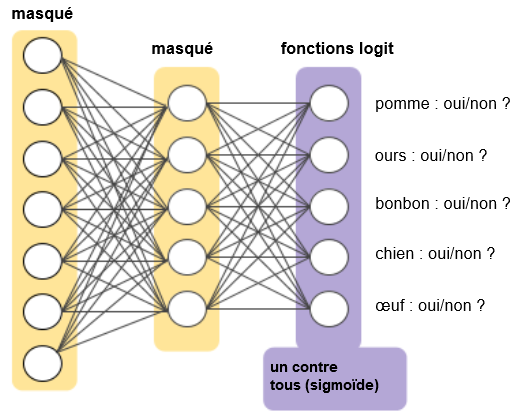
\includegraphics{./Capture_1.png} 
\end{center}

\subsection{Réseaux de neurones à classes multiples : Softmax}
Rappelez-vous que la régression logistique produit une décimale entre 0 et 1. Par exemple, un résultat de régression logistique de 0,8 pour un classificateur d'e-mails suggère que les chances qu'un e-mail soit indésirable sont de 80 \%, et les chances qu'il ne soit pas indésirable de 20 \%. De façon évidente, la somme des probabilités qu'un e-mail soit indésirable ou non est égale à 1.\\\\
\textbf{Softmax} étend cette idée à un monde à plusieurs classes. C'est-à-dire que \textbf{Softmax} attribue des probabilités décimales à chaque classe d'un problème à plusieurs classes. La somme de ces probabilités décimales doit être égale à 1. Cette contrainte supplémentaire permet de faire converger l'apprentissage plus rapidement qu'il ne le ferait autrement.\\\\
Par exemple, revenons à l'analyse de l'image de la Figure 1. Softmax pourra produire les probabilités suivantes qu'une image appartienne à une classe spécifique :

$$\begin{tabular}{| l |  r | }
	\hline			
	Classe & Probabilité \\
	\hline
	pomme & 0,001 \\
	ours & 0,04 \\
	friandises & 0,008 \\
	chien & 0,95 \\
	oeuf & 0,001 \\
	\hline  
\end{tabular}$$
\newpage
\textbf{Softmax} est mis en œuvre via une couche de réseau de neurones juste avant la couche du résultat. La couche Softmax doit comporter le même nombre de nœuds que la couche du résultat.
\begin{center}
	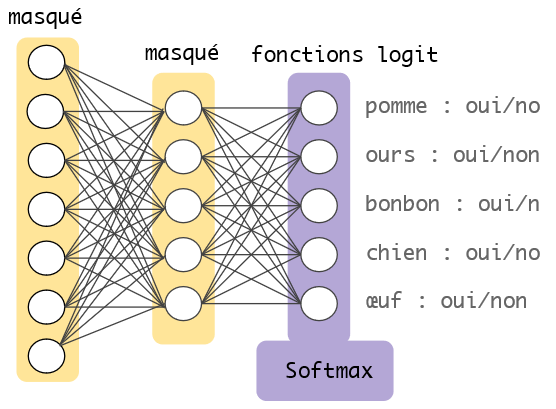
\includegraphics{./Capture_2.png} 
\end{center}
L'équation \textbf{Softmax} est la suivante : 
$$\bm{
	\mathbb{P}(y=j|x)=
	\frac{\exp(w_{j}^{T}x+b_{j})}
		{\sum_{k\in K}\exp(w_{k}^{T}x+b_{k})}
}$$
Notons que cette formule développe la formule de la régression logistique sur plusieurs classes.

\subsubsection{Options de Softmax}
Prenons les variantes de Softmax suivantes :\\
\begin{itemize}[label=$\Diamond$]
	\item \textbf{Softmax complet} est le \textbf{Softmax} dont nous avons parlé, c'est-à-dire le \textbf{Softmax} qui calcule une probabilité pour chaque classe possible.\\
	\item \textbf{L'échantillonnage de candidats} signifie que Softmax calcule une probabilité pour toutes les étiquettes positives, mais seulement pour un échantillon aléatoire d'étiquettes négatives. Par exemple, si nous souhaitons déterminer si une image d'entrée est un beagle ou un limier, il est inutile de fournir des probabilités pour chaque exemple "non chien".\\
\end{itemize}
\textbf{Softmax} complet est relativement économique lorsque le nombre de classes est petit, mais devient extrêmement coûteux lorsque le nombre de classes augmente. L'échantillonnage de candidats peut améliorer l'efficacité des problèmes qui comportent un grand nombre de classes.

\subsubsection{Une étiquette ou plusieurs étiquettes}
Softmax suppose que chaque exemple appartient exactement à une classe. Cependant, certains exemples peuvent appartenir simultanément à plusieurs classes.\\ Pour ces exemples :
\begin{itemize}[label=\textbullet]
	\item Vous ne pouvez pas utiliser Softmax.
	\item Vous devez vous appuyer sur les régressions logistiques.\\
\end{itemize}
Par exemple, supposons que vos exemples sont des images contenant exactement un élément : un fruit. \textbf{Softmax} peut déterminer la probabilité que cet élément soit une poire, une orange, une pomme, etc. Si vos exemples sont des images contenant toute sorte de choses (des saladiers contenant plusieurs types de fruits), alors vous devrez utiliser plusieurs régressions logistiques.


    \end{document}
    
